\documentclass[11pt,a4paper,twoside]{book} %scrbook book report
\usepackage{hyperref}  % Necesario para manejar los enlaces
\usepackage[
backend=biber,
style=apa,
%sorting=none,
backref=true,         % Habilitar backref
backrefstyle=none,    % Controla el formato de las referencias a las páginas
hyperref=true,         % Habilitar hyperref
]{biblatex}

% Add the ISSN field for journal articles
\DeclareBibliographyDriver{article}{%
	\usebibmacro{bibindex}%
	\usebibmacro{begentry}%
	\usebibmacro{author/editor+others/translator+others}%
	\setunit{\labelnamepunct}\newblock
	\usebibmacro{title}%
	\newunit
	\printlist{language}%
	\newunit\newblock
	\usebibmacro{byauthor}%
	\newunit
	\usebibmacro{journal+issuetitle}%
	\newunit
	\usebibmacro{byeditor+others}%
	\newunit
	\printfield{year}\newunit
	\printfield{volume}\newunit
	\printfield{number}\newunit
	\printfield{pages}\newunit
	\newunit\newblock
	\printfield{issn} % This will now include the ISSN field
	\newunit\newblock
	\usebibmacro{doi+eprint+url}%
	\newunit\newblock
	\usebibmacro{pageref}%
	\newunit\newblock
	\usebibmacro{related}%
	\usebibmacro{finentry}%
}

\addbibresource{own-bib.bib}



% Configuración de hyperref
\hypersetup{
	colorlinks=true,    % Habilita el coloreado de los enlaces
	linkcolor=blue,     % Color de los enlaces internos
	citecolor=blue,     % Color de las citas
	urlcolor=blue       % Color de los enlaces externos
}


% Essential packages
\usepackage{amsmath, amssymb, amsthm} % AMS Packages
\usepackage{graphicx,color}           % Packages for graphics and color
\usepackage{geometry}
\PassOptionsToPackage{printonlyused,smaller}{acronym}
\usepackage{acronym}
% Optional customization packages
\usepackage{lmodern}                  % Custom fonts
\usepackage[T1]{fontenc}              % Ensure correct font encoding
\usepackage{mathptmx}              % Times New Roman Font accross the document

\usepackage{subfigure}
%\usepackage{subcaption}
\usepackage{wrapfig}
\usepackage{multirow}

\usepackage{multicol}

\usepackage{url}

\usepackage{listings}

%\usepackage{xcolor}

\definecolor{codegreen}{rgb}{0,0.6,0}
\definecolor{codegray}{rgb}{0.5,0.5,0.5}
\definecolor{codepurple}{rgb}{0.58,0,0.82}
\definecolor{backcolour}{rgb}{0.95,0.95,0.92}

\lstdefinestyle{mystyle}{
	backgroundcolor=\color{backcolour},   
	commentstyle=\ttfamily\color{codegreen},
	keywordstyle=\color{magenta},
	numberstyle=\tiny\color{codegray},
	stringstyle=\color{codepurple},
	basicstyle=\footnotesize,
	breakatwhitespace=false,         
	breaklines=true,                 
	captionpos=b,                    
	keepspaces=true,                 
	numbers=left,                    
	numbersep=5pt,                  
	showspaces=false,                
	showstringspaces=false,
	showtabs=false,                  
	tabsize=2
}


\lstset{style=mystyle}
\lstset{language=Python}

% Customising chapter headings - sectsty.pdf
\usepackage{sectsty}
\chapterfont{\Large\sc\centering}
\chaptertitlefont{\centering}
\subsubsectionfont{\centering}

\usepackage[hang, small, bf, margin=0pt, tableposition=bottom]{caption}
\setlength{\abovecaptionskip}{10pt}   % Custom captions

\captionsetup{
	justification=justified, % Center the caption label and first line
	format=plain, % Standard format
	singlelinecheck=false, % Disable single line centering
	indention=0pt
}

% Tables
\usepackage[table]{xcolor}
\usepackage{colortbl}

\usepackage{todonotes}

\newcommand{\mc}[2]{\multicolumn{#1}{c}{#2}}
\definecolor{Gray}{gray}{0.83}

\newcolumntype{x}{>{\columncolor{Gray}}c}
\newcolumntype{y}{>{\columncolor{white}}c}

% Page layout
\parindent 0pt
\parskip 1ex
\renewcommand{\baselinestretch}{1.49}
\numberwithin{equation}{section}
\renewcommand{\bibname}{References}
\renewcommand{\contentsname}{Contents}
\pagenumbering{roman}


\newcommand{\acrolabel}[1]{\makebox[3cm][l]{\textbf{#1}}}
\newenvironment{acronyms}{\begin{list}{}{\renewcommand{\makelabel}{\acrolabel}}}{\end{list}}

% \includeonly{tex/chapter1}          % Option to generate specific chapters

% Customising headers - fancyhdr.pdf
\usepackage{fancyhdr}
\pagestyle{fancy}
\rhead{}
\lhead{\nouppercase{\textsc{\leftmark}}}
\renewcommand{\headrulewidth}{0pt}
\makeatletter
\renewcommand{\chaptermark}[1]{\markboth{\textsc{\@chapapp}\ \thechapter:\ #1}{}}
\makeatother


% Hyperreferencing and citations
\usepackage{hyperref}
\hypersetup{
	colorlinks,
	citecolor=blue,
	filecolor=blue,
	linkcolor=blue,
	urlcolor=blue
}

% Section symbol
\usepackage{cleveref}
\crefname{section}{\S}{\S\S}
\Crefname{section}{\S}{\S\S}
\crefname{subsection}{\S}{\S\S}
\Crefname{subsection}{\S}{\S\S}

% packages from lymnaea paper
\usepackage{tabu}
\usepackage{adjustbox}
\usepackage{booktabs}
\usepackage{./styles/nust}

\graphicspath{{./img/}{./figs/}}

\title{Characterization of the sequential nature of neuronal dynamics: Experimental recordings, computational models and novel stimulation neurotechnology}

%\subtitle{A sub-title}

\author{Alicia Garrido Peña}

\degree{\EPS} % MSCSE, MSCCS %% Degree Title and It's abbreviation
\school{\EPS} %SChool abbreviation and Full Name

\adviser{Pablo Varona Martínez}

\regno{Doctorado en Ingeniería Informatica y Telecomunicaciones}
\adviserAffiliation{Departamento Ingeniería Informática}

\date{August 2024}

% \setcounter{tocdepth}{2}
% \setstretch{1.1}
% \linespread{1.1}


\geometry{margin=1in,top=1in, bottom=1in, includefoot, headheight=13.6pt}

\begin{document}
	
	
	%\begin{appendix}
	\centering\huge\textbf{{List of Publications Related to the PhD Thesis}}\\
	\large{\textbf{PhD Candidate:} Alicia Garrido Peña}\\
	\large{\textbf{Advisor:} Pablo Varona Martinez}
	% \section{Research Publications}
	
	\begin{refsection}[own-bib.bib]
		\nocite{*}
		
		\printbibliography[heading={subbibliography},title={Journal Publications},keyword=journal]
		
		\printbibliography[heading={subbibliography},title={International Conference Contributions},keyword=conference]
		
%		\printbibliography[heading={subbibliography},title={Conference Contributions},type=article,keyword=conference]
		
		
	\end{refsection}
	%\chapter{Supplementary figures for chapter 4}
	%
	%\begin{figure}[htbp]
	\centering
	\includegraphics[width=0.9\textwidth]{./invariants/data/MODEL/n1m_driven/images/3phases/_output_pairplot_reset.png}
	\caption{\textbf{N1M stimulation}:Pairplot of the invariants no reset within cycles. Lower triangle represents the intervals within the same cycle. Upper triangle represents the intervals of one cycle within the next cycle. }
	\label{fig:N1M stimulation pairplot reset}
\end{figure}

\begin{figure}[htbp]
	\centering
	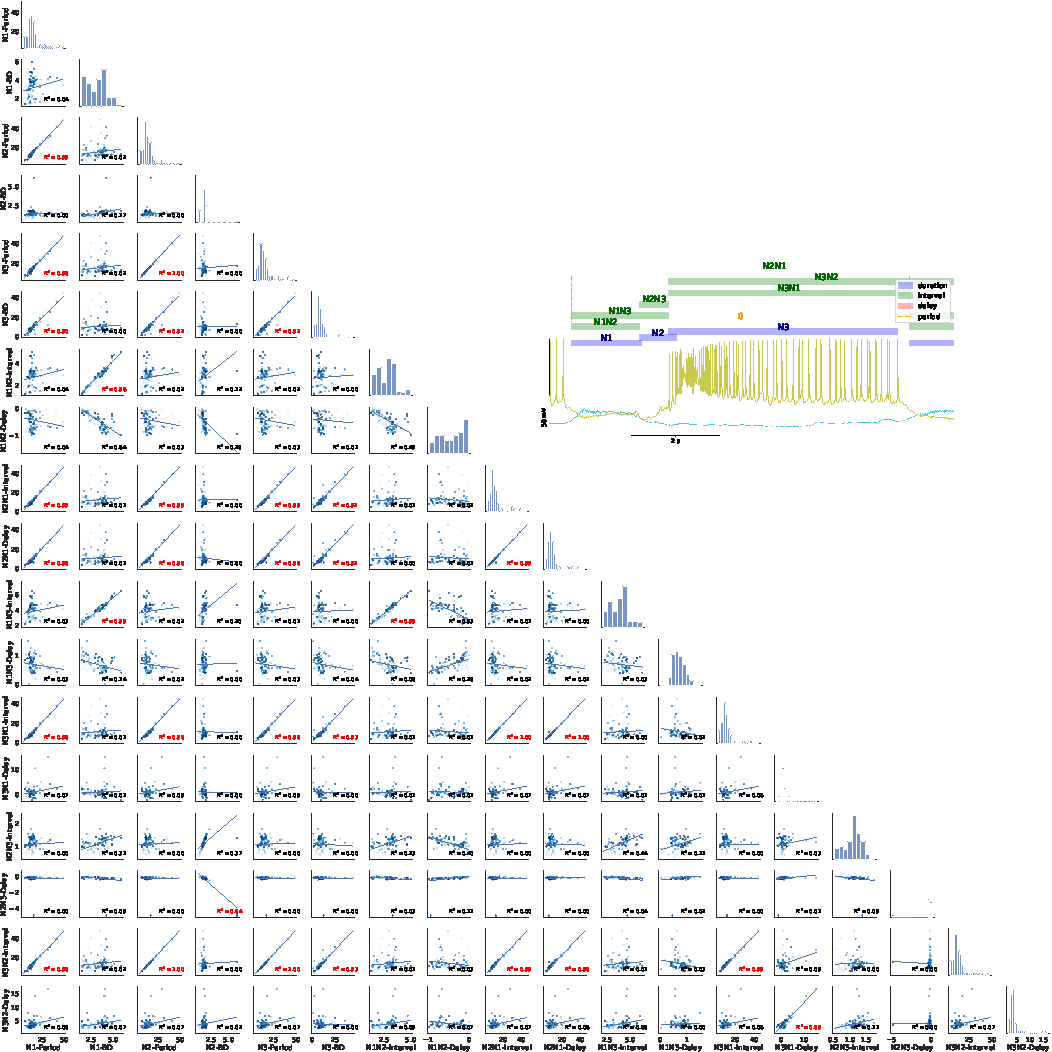
\includegraphics[width=\textwidth]{./img/invariants/data/SUSSEX/prep2/images/3phases/panel_with_pairplot.pdf}
	\caption{\textbf{Spontaneous case 1}: Panel of intervals distribution and dynamical invariants for the three phases in the CPG for spontaneous activity.}
	\label{fig:prep2 pairplot invariants}
\end{figure}



\begin{figure}[htbp]
	\centering
	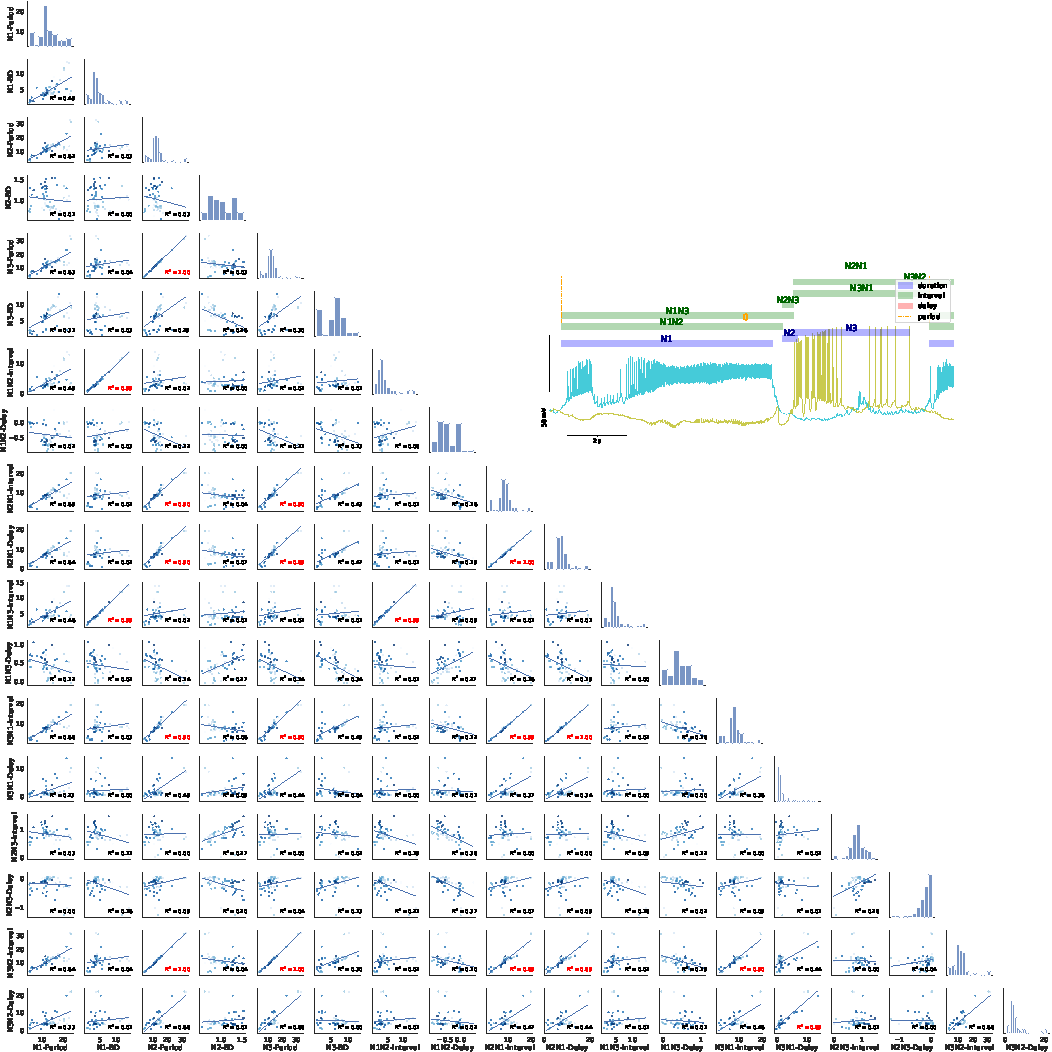
\includegraphics[width=0.9\textwidth]{./img/invariants/data/SUSSEX/prep3/images/3phases/panel_with_pairplot.pdf}
	\caption{\textbf{Spontaneous case 2}: Panel of intervals distribution and dynamical invariants for the three phases in the CPG for spontaneous activity.}
	\label{fig:prep3 invariants pairplot}
\end{figure}


\begin{figure}[htbp]
	\centering
	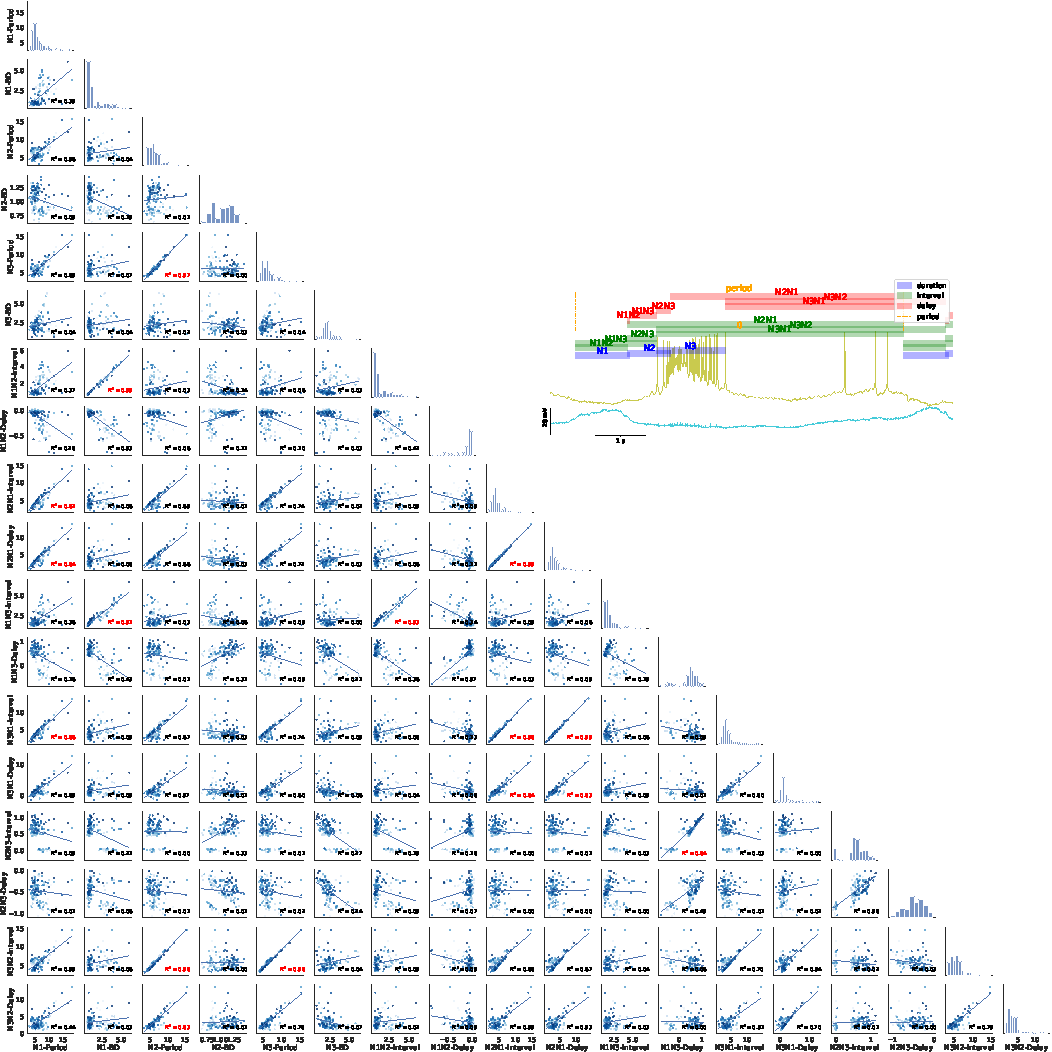
\includegraphics[width=\textwidth]{./img/invariants/data/SUSSEX/prep1/images/3phases/panel_with_pairplot.pdf}
	\caption{\textbf{Spontaneous case 3}: Panel of intervals distribution and dynamical invariants for the three phases in the CPG for spontaneous activity.}
	\label{fig:prep1 invariants pairplot}
\end{figure}

% sale mal, probablemente pq el fin e inicio de n2v es idéntico
%\begin{figure}[htbp]
%	\centering
%	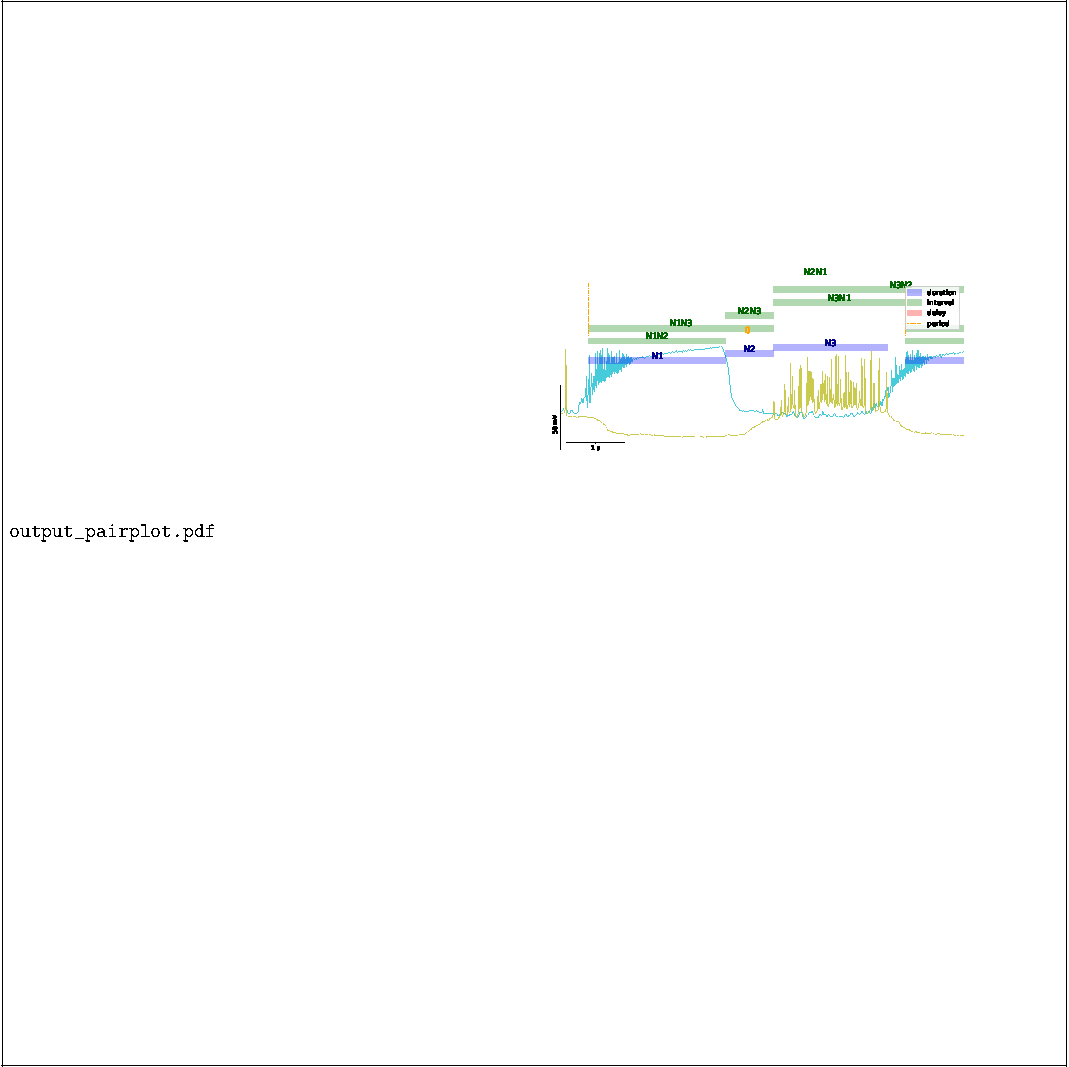
\includegraphics[width=0.9\textwidth]{./img/invariants/data/SUSSEX/CV1a_driven1/images/3phases/panel_with_pairplot.pdf}
%	\caption{\textbf{CV1a driven case1}: Panel of intervals distribution and dynamical invariants for the three phases in the CPG under CV1a stimulation.}
%	\label{fig:cv1a 1 3phases pairplot}
%\end{figure}
%

\begin{figure}[htbp]
	\centering
	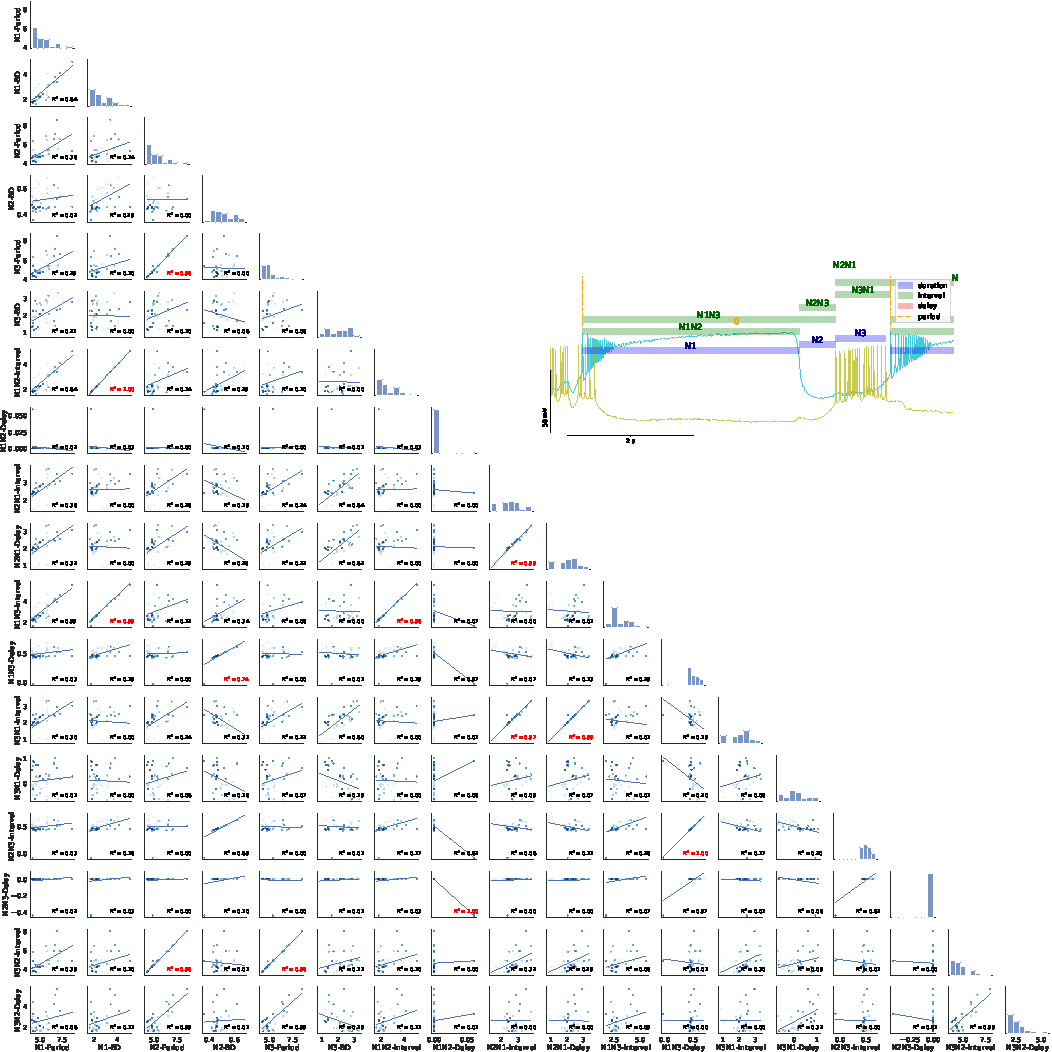
\includegraphics[width=0.9\textwidth]{./img/invariants/data/SUSSEX/CV1a_driven4/images/3phases/panel_with_pairplot.pdf}
	\caption{\textbf{CV1a driven case 4}: Panel of intervals distribution and dynamical invariants for the three phases in the CPG under CV1a stimulation.}
	\label{fig:cv1a 4 3phases pairplot}
\end{figure}



\begin{figure}
	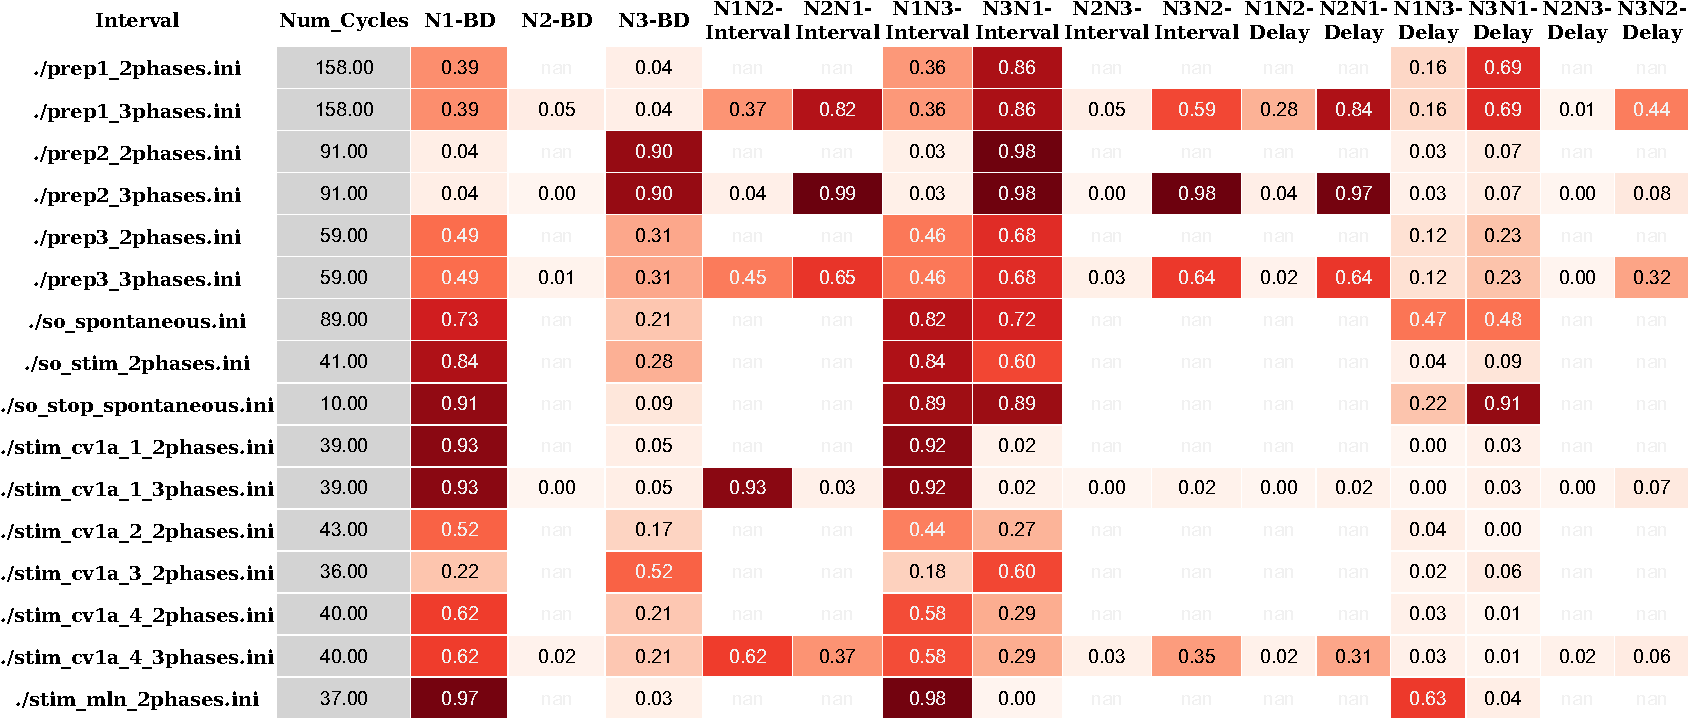
\includegraphics[width=\textwidth]{./img/invariants/styled_table_invariants_r-squared.pdf}
	\caption{Table of $R^2$ values for the linear regression between the period and each interval for all experimental recordings showed in this section.}
	\label{fig:R2 table}
\end{figure}

	
	\pagenumbering{gobble}
	%% The first official use of the word "Neuroscience" may be in 1962 with Francis O. Schmitt's "Neuroscience Research Program", which was hosted by the Massachusetts Institute of Technology1
% . Therefore, it is not clear who coined the term "neuroscience".

The Neuron. CELL AND MOLECULAR BIOLOGY
IRWIN B. LEVITAN
LEONARD K. KACZMAREK
"how many neurons are involved in the control of a scpecific behavior, where are located and how they are connected. 
All play roles in the output of that circuit. 

Physiologtsts, biochemists, and anatomists  .... Neuroscience is already a mature discipline in its own right. 



Santiago Ramón y Cajal made significant contributions to the field of neuroscience. Here are some of his major contributions:

    Neuron Doctrine: Cajal's greatest contribution to neuroscience is the idea of the "neuron doctrine," which he proposed and supported with evidence. He showed that the nervous system comprises individual cells called neurons, which connect to each other at small, specialized contact zones called synapses. He also demonstrated that a single nerve cell typically possesses three anatomically distinct structures3
    .
    Staining Techniques: Cajal developed staining techniques that allowed him to visualize the structure of the nervous system with exquisite precision. He used these techniques to make many discoveries about the structure and function of neurons1
    .
    Dynamic Polarization: Cajal proposed the Law of Dynamic Polarization, which describes the directional flow of information in the nervous system. According to this law, information flows from the dendrites of a neuron to its cell body and then to its axon6
    .
    Comparative Studies: Cajal conducted extensive comparative studies of the nervous system using material from humans, dogs, cats, rodents, birds, and reptiles. These studies led him to discover novel nuclei and cell types and to reorganize the ideas regarding the connections between neural regions and nuclei6
    .
    Meticulous Artwork: Cajal left behind a vast collection of meticulous and beautiful artwork that captures our understanding of the brain in his time. His drawings are still reproduced in neuroscience textbooks today2
    .

Overall, Cajal's contributions to neuroscience laid the foundations of modern neuroscience and continue to be valuable today.


Neuron- Signalling in the Brain. 
1840, Jacob Schleiden and Theodor Schwann --> Cells definition

Neuron. Three structural elements specific from neurons: axon, dendrites and synapse. 



Adapt models table from
https://www.sciencedirect.com/science/article/pii/S0896627319304441 Figure 2A:
\begin{figure}
    \centering
    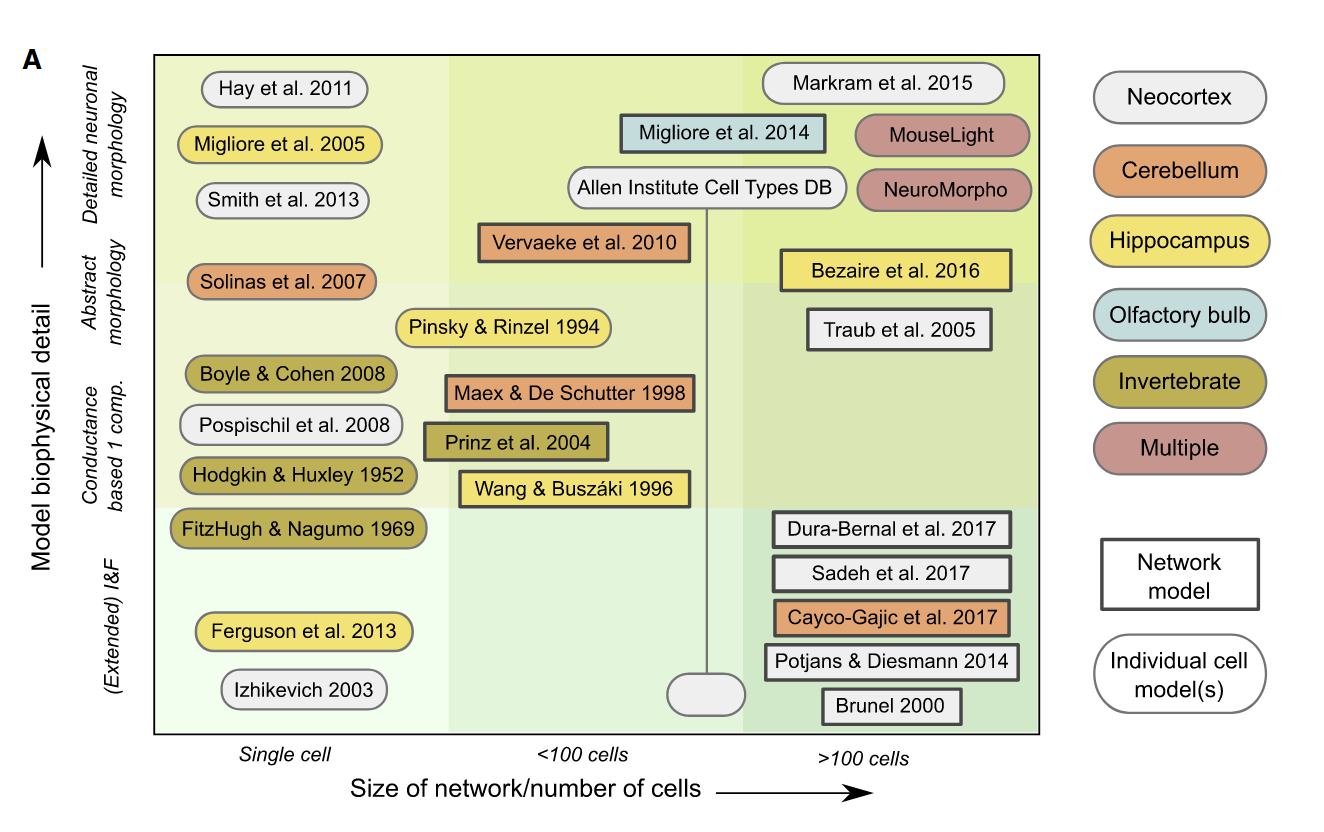
\includegraphics[width=\textwidth]{misc/models-table.png}
    \caption{Caption}
    \label{fig:models-table}
\end{figure}

Lotka-Volterra; Ginsburg-Landau
	% %!TEX root = ../_thesis.tex
\begin{table}[!ht]
\footnotesize
\begin{adjustbox}{width=\linewidth,center}
\begin{tabular}{p{0.6cm}p{9cm}p{0.6cm}}
% \multicolumn{3}{r}{Annex 'A'} \\
\multicolumn{3}{r}{Office Order: 0986/29/ACB/SEECS} \\
\multicolumn{3}{r}{Date  \today}                                          \\
\multicolumn{3}{c}{\textbf{Th.ECL (MS Thesis   Evaluation Check List)}}   \\\midrule
\multicolumn{3}{|l|}{Student  Name:}                                                                                                                                                     \\ \midrule
\multicolumn{3}{|l|}{Registration:}                                                                                                                                                      \\ \midrule
\multicolumn{3}{|l|}{\textbf{Cover and title   page of the thesis}}                                                                                                                      \\ \midrule
\multicolumn{1}{|l|}{T1.} & \multicolumn{1}{l|}{Student's name and registration   number is written.}                                                            & \multicolumn{1}{l|}{} \\ \midrule
\multicolumn{1}{|l|}{T2.} & \multicolumn{1}{l|}{Supervisor's name is   mentioned.}                                                                               & \multicolumn{1}{l|}{} \\ \midrule
\multicolumn{1}{|l|}{T3.} & \multicolumn{1}{l|}{Title of the degree   is written correctly.}                                                                     & \multicolumn{1}{l|}{} \\ \midrule
\multicolumn{1}{|l|}{T4.} & \multicolumn{1}{l|}{University and   school's name are written correctly.}                                                           & \multicolumn{1}{l|}{} \\ \midrule
\multicolumn{1}{|l|}{T5.} & \multicolumn{1}{l|}{Date of   completion/defense (only year and month) is mentioned.}                                                & \multicolumn{1}{l|}{} \\ \midrule
\multicolumn{3}{|l|}{\textbf{Style and formatting issues}}                                                                                                                               \\ \midrule
\multicolumn{1}{|l|}{S1.} & \multicolumn{1}{l|}{Consistent font (Times New Roman) is   used throughout the thesis.}                                              & \multicolumn{1}{l|}{} \\ \midrule
\multicolumn{1}{|l|}{S2.} & \multicolumn{1}{l|}{Page numbering is   done appropriately.}                                                                         & \multicolumn{1}{l|}{} \\ \midrule
\multicolumn{1}{|l|}{S3.} & \multicolumn{1}{l|}{Figures are readable   and are aligned correctly.}                                                               & \multicolumn{1}{l|}{} \\ \midrule
\multicolumn{1}{|l|}{S4.} & \multicolumn{1}{l|}{Captions for tables   and figures use consistent format and style.}                                              & \multicolumn{1}{l|}{} \\ \midrule
\multicolumn{1}{|l|}{S5.} & \multicolumn{1}{l|}{Table of   Contents/Figures/Tables follow proper indentation/styling.}                                           & \multicolumn{1}{l|}{} \\ \midrule
\multicolumn{1}{|l|}{S6.} & \multicolumn{1}{l|}{Chapter name and   numbering follows consistent style.}                                                          & \multicolumn{1}{l|}{} \\ \midrule
\multicolumn{3}{|l|}{\textbf{References/Bibliography}}                                                                                                                                   \\ \midrule
\multicolumn{1}{|l|}{R1.} & \multicolumn{1}{l|}{References are   sorted on last name of authors (or in the order of citation in the text).}                      & \multicolumn{1}{l|}{} \\ \midrule
\multicolumn{1}{|l|}{R2.} & \multicolumn{1}{l|}{References follow   consistent style such as ACM or IEEE-Tran.}                                                  & \multicolumn{1}{l|}{} \\ \midrule
\multicolumn{1}{|l|}{R3.} & \multicolumn{1}{l|}{Mandatory slots of   references are filled correctly (such as Author, Title, Journal, Year).}                    & \multicolumn{1}{l|}{} \\ \midrule
\multicolumn{3}{|l|}{\textbf{General Issues}}                                                                                                                                            \\ \midrule
\multicolumn{1}{|l|}{G1.} & \multicolumn{1}{l|}{Certificate of Originality signed by   the student is present.}                                                  & \multicolumn{1}{l|}{} \\ \midrule
\multicolumn{1}{|l|}{G2.} & \multicolumn{1}{l|}{Plagiarism   report (from Euphorus) signed by supervisor is presented along with the   thesis.}                  & \multicolumn{1}{l|}{} \\ \midrule
\multicolumn{1}{|l|}{G3.} & \multicolumn{1}{l|}{Thesis is submitted   within allowed time span for completion of thesis.}                                        & \multicolumn{1}{l|}{} \\ \midrule
\multicolumn{3}{|l|}{\textbf{Abstract (Note:   This section covers only the abstract of the thesis)}}                                                                                    \\ \midrule
\multicolumn{1}{|l|}{A1.} & \multicolumn{1}{l|}{There are no typing or grammatic   mistakes in the abstract.}                                                    & \multicolumn{1}{l|}{} \\ \midrule
\multicolumn{1}{|l|}{A2.} & \multicolumn{1}{l|}{Problem statement is   clearly mentioned.}                                                                       & \multicolumn{1}{l|}{} \\ \midrule
\multicolumn{1}{|l|}{A3.} & \multicolumn{1}{l|}{Background to problem   statement is also explained.}                                                            & \multicolumn{1}{l|}{} \\ \midrule
\multicolumn{1}{|l|}{A4.} & \multicolumn{1}{l|}{Startling statement   (preferably a paragraph) about the thesis/hypothesis is present.}                          & \multicolumn{1}{l|}{} \\ \midrule
\multicolumn{1}{|l|}{A5.} & \multicolumn{1}{l|}{Implication of the   startling statement is demonstrated briefly.}                                               & \multicolumn{1}{l|}{} \\ \midrule
\multicolumn{3}{|l|}{\textbf{Results, Evaluation, and Conclusion}}                                                                                                                       \\ \midrule
\multicolumn{1}{|l|}{E1.} & \multicolumn{1}{l|}{Research is   validated either empirically or analytically (Note: This doesn’t cover   quality of the results).} & \multicolumn{1}{l|}{} \\ \midrule
\multicolumn{1}{|l|}{E2.} & \multicolumn{1}{l|}{Outcome of this   thesis is contrasted with other similar research initiatives.}                                 & \multicolumn{1}{l|}{} \\ \midrule
\multicolumn{1}{|l|}{E3.} & \multicolumn{1}{l|}{Significance of this   research is discussed in appropriate length.} \\ \midrule
\end{tabular}
\end{adjustbox}
\end{table}
	
	
	%\end{appendix}
\end{document}
